\documentclass[11pt]{article}
\usepackage[utf8]{inputenc}
\usepackage[brazil]{babel}

\usepackage{float}
\usepackage{amsmath}
\usepackage{amssymb}
\usepackage{graphicx}
\newtheorem{theorem}{Teorema}[section]

\title{MO420 - TP de Planos de Cortes}
\author{RA009206 - Luís Guilherme Fernandes Pereira \\
RA044072 - Igor Ribeiro de Assis}
\date{Trabalho 3 - 1o semestre de 2009}

\begin{document}
\maketitle

\section{Introdução}

Neste trabalho prático, estudamos o problema de planos de cortes e
Branch and Cut, implementamos essa técnica no resolvedor XPress e
usamo-la para resolver o problema de \emph{minimum stabbing number}
(STAB).

\section{Formulação}

A seguinte formulação para o problema STAB foi utilizada.

\begin{align}
  min & \hspace{8pt}y\\
  s.a & \hspace{2pt}\sum_{e \in \delta (i)}{x_e} = 1 \label{grau} \\
      & \sum_{e \in E(S)}{x_e} \le (|S|-1)/2, \hspace{4pt} \forall S
  \subset P, \hspace{4pt} |S|
  \hspace{4pt} impar \label{exp} \\
      & \sum_{e \in I(r_{ij})}{x_e} \le y, \forall (i,j) \in N \times N,
    i < j \label{inter}
\end{align}

As restrições \eqref{grau} e \eqref{exp} são as restrições do problema
de emparelhamento perfeito (note que se a restrição de grau fosse do
tipo $\le$ teríamos a formulação emparelhamento máximo). As restrições
\eqref{grau} são restrições de grau e garantem que em cada vértice
exatamente uma aresta incidente nele tem o valor $x_e = 1$. As do tipo
\eqref{exp} embora não necessárias na formulação inteira do problema
do emparelhamento, ao se resolver o programa linear relaxado
correspondente elas evitam soluções com valores fracionários como na
figura \ref{fig:ciclo_impar}, e mais, são necessárias na descrição da
envoltória convexa [REFERÊNCIA DO ARTIGO AQUI].

Intuitivamente essas restrições dizem que para todo conjunto ímpar de
vértices, deve exister algum vértice ``casando'' com alguem de fora do
conjunto, observe que é importante que a $|S|$ seja ímpar caso
contrário estaríamos excluindo soluções válidas.

A variável $y$, utilizada no último grupo de restrições e na função
objetivo corresponde a um limite superior para o número de
intersecções de uma reta (das retas consideradas tendo em vista a
proposição $1$) com os segmentos do emparelhamento perfeito
encontrado, ou seja, a váriavel $y$ é um limite superior para o
$sn(M)$. Como o problema é de minimização da variável $y$, em qualquer
solução ótima no mínimo uma restrição do tipo \eqref{inter} será
satisfeita na igualdade.

\begin{figure}[H]
\centering
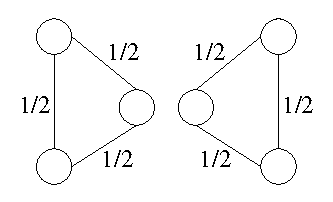
\includegraphics[scale=0.50]{ciclos}
\caption{Solução inválida do emparelhamento satisfazendo as restrições
  de grau}
\label{fig:ciclo_impar}
\end{figure}

Note que o número de restrições do tipo \eqref{exp} é exponencial,
portanto não é possível utilizar essa formulação com todas as
restrições é necessário um algoritmo de \emph{branch-and-cut}

Vejamos agora restrições alternativas para as do tipo \eqref{exp}, que
ao invés de somarem sobre as arestas do conjunto $S$, somam sobre as
arestas do corte cuja praia é $S$.

\begin{align}
  \sum_{e \in S}{x_e} \ge 1, \hspace{4pt}|S|\hspace{4pt} impar \label{corte}
\end{align}

Vamos mostrar que \eqref{corte} e \eqref{exp} são equivalentes.

Fixe um conjunto $S$ e seja $x^*$ uma solução do problema linear acima
que não satisfaz as restrições \eqref{exp}. Temos:

\begin{align}
  2\sum_{e \in E(S)}x_e^* > (|S| - 1)
\end{align}

Para o conjunto $S$,

\begin{align}
  \sum_{e \in \delta (S)}x_e^* = \sum_{i \in S}\sum_{e \in \delta
    (i)}x_e^* - 2\sum_{e \in E(S)}x_e^* < \sum_{i \in S}\sum_{e in
    \delta (i)}x_e^* - (|S| - 1)
\end{align}

Mas pelo fato de $x^*$ satisfazer as restrições de grau temos $\sum_{i
  \in S}\sum_{e \in \delta (i)}x_e^* = |S|$, portanto, $\sum_{e \in
  \delta (S)} < 1$, e $x^*$ não satisfaz \eqref{corte}. De maneira
análoga obtemos que se uma solução não satisfaz \eqref{corte} não
satisfaz \eqref{exp}.

Suponha agora que $x^*$ é uma solução válida para \eqref{exp}, então:

\begin{align}
  2\sum_{e \in E(S)}x_e^* \le (|S| - 1)
\end{align}

E,

\begin{align}
  \sum_{e \in \delta (S)}x_e^* = \sum_{i \in S}\sum_{e \in \delta
    (i)}x_e^* - 2\sum_{e \in E(S)}x_e^* \ge \sum_{i \in S}\sum_{e in
    \delta (i)}x_e^* - (|S| - 1)
\end{align}

Portanto, como $x^*$ satisfaz as restrições de grau, $\sum_{e \in
  \delta (S)} \ge 1$, como queríamos.

\end{document}
